%%%%%%%%%%%%%%%%%%%%%%%%%%%%%%%%%%%%%%%%%%%%%%%%%%%%%%%%%%%%%%%%%%
%%%%%%%% ICML 2017 EXAMPLE LATEX SUBMISSION FILE %%%%%%%%%%%%%%%%%
%%%%%%%%%%%%%%%%%%%%%%%%%%%%%%%%%%%%%%%%%%%%%%%%%%%%%%%%%%%%%%%%%%

% Use the following line _only_ if you're still using LaTeX 2.09.
%\documentstyle[icml2017,epsf,natbib]{article}
% If you rely on Latex2e packages, like most moden people use this:
\documentclass{article}

% use Times
\usepackage{times}
% For figures
\usepackage{graphicx} % more modern
%\usepackage{epsfig} % less modern
\usepackage{subfigure} 

% For citations
\usepackage{natbib}

% For algorithms
\usepackage{algorithm}
\usepackage{algorithmic}

% As of 2011, we use the hyperref package to produce hyperlinks in the
% resulting PDF.  If this breaks your system, please commend out the
% following usepackage line and replace \usepackage{icml2017} with
% \usepackage[nohyperref]{icml2017} above.
\usepackage{hyperref}

% Packages hyperref and algorithmic misbehave sometimes.  We can fix
% this with the following command.
\newcommand{\theHalgorithm}{\arabic{algorithm}}

% Employ the following version of the ``usepackage'' statement for
% submitting the draft version of the paper for review.  This will set
% the note in the first column to ``Under review.  Do not distribute.''
\usepackage{icml2017} 

% Employ this version of the ``usepackage'' statement after the paper has
% been accepted, when creating the final version.  This will set the
% note in the first column to ``Proceedings of the...''
%\usepackage[accepted]{icml2017}

\usepackage{supertabular,booktabs}
\usepackage{amsmath}
\usepackage{amssymb}

% The \icmltitle you define below is probably too long as a header.
% Therefore, a short form for the running title is supplied here:
\icmltitlerunning{Adversarial Attacks on Image Recognition}

\begin{document}
	\icmltitle{Adversarial Attacks on Image Recognition}
	\icmlkeywords{Adversarial Attacks, machine learning, ICML}
	\begin{abstract}
	This paper extends the work done by Papernot et al. in \yrcite{papernot3} on adversarial attacks on image recognition. We investigated whether a reduction in feature dimensionality using principle component analysis (PCA) can maintain a comparable level of misclassification success while increasing computational efficiency. We attacked black-box image classifiers trained on the MNIST dataset by forcing the oracle to misclassify images that were modified with small perturbations. The method we used was two-fold: the target classifier was imitated with a substitute logistic regression model and then the adversarial samples were generated off of the substitute model \cite{papernot3}. The results show that reasonable misclassification rates of $\sim 70\%$ with reduced computation time can be achieved for a PCA-reduced feature set utilizing the Papernot adversarial crafting algorithm.
\end{abstract}
	\section{INTRODUCTION}

Machine learning techniques, coupled with data, are used to solve a multitude of high-dimensional problems with great success, such as those in the area of image recognition. For instance, image recognition is employed in self-driving cars to navigate on the roads. However, research has shown that these machine learning models are not robust to adversarial attacks and can be exploited by injecting specifically designed samples to training data or by creating test samples based on the decision boundary of the algorithm to misguide the classification result. For example, Papernot et. al. showed that it is possible to craft an image that would appear to be a stop sign but would be classified as a yield sign by some class of deep neural networks \yrcite{papernot1}. Furthermore, Papernot et. al. also found that the perturbation technique they used to construct such adversarial samples is applicable to a variety of other classifiers, such as support vector machines and logistic regression \yrcite{papernot3}. These findings demonstrated that machine learning systems are susceptible to malicious attacks. One such example would be to alter the image of road signs received by autonomous driving systems in order to manipulate the behaviour of target vehicles, which could lead to dire consequences. Thus, understanding the vulnerabilities of machine learning systems and the methods to exploit them is crucial for application of machine learning in practical settings.
	\section{LITERATURE} \label{sec:literature}

Papernot et al. in \yrcite{papernot3} described the following two step approach during adversarial sample creation for a black-box machine learning algorithm referred to as the 'oracle' from this point forward:
% should we mention the Papernot method here?
\begin{enumerate}
\item \label{step1} Train a substitute model utilizing as few calls to the oracle as possible.  
\item \label{step2} Craft adversarial samples using either the fast gradient sign (FGS) method \cite{papernot3} or the Papernot method \cite{papernot2}. 
\end{enumerate}

In \cite{papernot3}, the logistic regression (LR) and deep neural network (DNN) substitute models had the highest cross-technique transferability, indicating that adversarial techniques crafted by these models would be misclassified by oracles with a different machine learning algorithm structure (e.g. SVM, k-nearest neighbours, etc.) with a high success rate. This means that given a black-box oracle, a choice of LR or DNN substitute model should create effective adversarial samples. These substitute models must be trained on datasets obtained by querying the oracle. Papernot et al. started with a small training set, and utilized Jacobian-based dataset augmentation to increase the number of samples by querying the oracle on the datapoints that exhibit the most change. This method is described by the following formula \cite{papernot3}:
\begin{equation} \label{eq:1}
	S_{\rho+1} = \left\{\vec{x} + \lambda_{\rho}\textbf{sgn}(J_{f}[O[(\vec{x})] : \vec{x} \in S_{\rho})\right\} \cup S_{\rho}
\end{equation}
where $S$ is the training set, $\vec{x}$ is a sample in $S$, $O(\vec{x})$ is the label given to sample $\vec{x}$ by the oracle, $J_{f}$ is the Jacobian matrix of the substitute model $f$, and $\lambda$ is the tuneable step-size parameter. At each iteration $\rho$, the training set is augmented by utilizing Equation \ref{eq:1}. The oracle is then called to obtain the labels for the new training dataset, and subsequently a new substitute model $f$ is trained. Furthermore, in \cite{papernot3}, the periodic step size (PSS) technique was introduced to improve the approximation of the oracle with the substitute model by multiplying the $\lambda$ parameter by $-1$ when the Jacobian augmentation method no longer lead to a significant improvement in the substitute model. Then, $\lambda_{\rho}$ is defined as
\begin{align}
	\lambda_{\rho} = \lambda(-1)^{\left \lfloor \frac{\rho}{\tau} \right \rfloor}    
\end{align}
where $\tau$ is the number of iterations after which the Jacobian augmentation method is no longer effective. However, the oracle should not be queried excessively to avoid raising suspicion. To diminish the calls to the oracle, reservoir sampling (RS) was utilized. Reservoir sampling selects $\kappa$ randomly generated new samples after $\sigma$ iterations have been completed normally. This decreases the number of calls to the oracle from $n(2^{\rho})$ to $n(2^{\sigma}) + \kappa (\rho-\sigma)$ \cite{papernot3}. Papernot et al. found that a Jacobian augmentation method combined with PSS and RS produced substitute models that approximated the oracle model successfully. 

The purpose of this project is to extend the work done by Papernot et al. in \yrcite{papernot3} on adversarial attacks in image recognition. We investigated whether a reduction in feature dimensionality during adversarial sample crafting improved computational efficiency, while maintaining a comparable level of success in misclassification of the adversarial samples. We formed an attack on an oracle with a training set unknown to the substitute model by forcing the oracle to misclassify images that were modified with white noise undetectable to humans.
	\section{DATASET}
Since our work extends that done by Papernot et al. in \yrcite{papernot3, papernot1}, we utilize the same dataset cited in his papers, which is the MNIST dataset. This ensures the validity of our results. The MNIST hand-written digit dataset of $28 \times 28$ pixel images contains $50,000$ training, $10,000$ validation, and $10,000$ test greyscale images \cite{mnist}. 

%The MNIST dataset is used to replicate the results of transferability between machine learning algorithms in crafting adversarial samples outlined in \cite{papernot3}, ensuring the validity of our approach.

%The MNIST dataset is used to replicate the results of transferability between machine learning algorithms in crafting adversarial samples outlined in \cite{papernot3}. This is done in order to ensure that the experiment performed in this paper is comparable to the work done in \cite{papernot3}. Then image feature reduction was performed to investigate the effect of reduced dimensionality when training the substitute model on the success of adversarial samples in by-passing the oracle.
	\section{METHODS}

\subsection{Black-Box Models}

To investigate the effectiveness of Papernot's approach outlined in Section \ref{sec:literature} with image feature reduction, a set of three black-box models were selected to act as the oracle for comparison. We chose the logistic regression (LR), support vector machine (SVM), and k-nearest neighbours (kNN) models due to simplicity of implementation and Papernot's use of these models in \cite{papernot3}. We implemented the LR and kNN models as described in the course notes \cite{coursenotes}. For SVM, we used the \texttt{fitcsvm} function in Matlab \cite{matlab}. Since SVMs are binary classifiers, to construct a multiclass classifier, we built an ensemble of one-versus-one classifiers for each pair of classes. The class assigned to a sample is the one that was selected by the majority of the classifiers \cite{multiclasssvm}. The models were trained on the MNIST $50,000$ image sample set, and tested on $10,000$ samples in the test set. The performance of each of these oracle models is shown in Table \ref{tab:oracles}. All models achieved a success rate of $\sim 90 \%$, deeming them sufficiently accurate to utilize as the black-box oracles in experiment.

\begin{table}[h]
\begin{center}
\begin{tabular}{ccc}
\toprule
LR & SVM & kNN\\
\midrule \midrule
87.5 & 93.9 & 96.7 \\
\bottomrule
\end{tabular}
\end{center}
\caption{Percentage of the test set that each model classified correctly.}
\label{tab:oracles}
\end{table}

\subsection{Logistic Regression Substitute Model}

An LR substitute model was chosen for this experiment due to its high cross transferability to other models \cite{papernot3}. This model was trained as described in Section \ref{sec:literature} utilizing Jacobian-based augmentation combined with PSS and RS. However, we found the Jacobian used in \cite{papernot3} to be incorrect. Instead, for an LR model $f$ described by the equation as in \cite{papernot3}

\begin{equation} \label{LR_prob}
	f: \vec{x} \rightarrow \Bigg[ \frac{e^{\vec{w}_{j}\vec{x}}}{\sum_{l=1}^{N}e^{\vec{w}_{l}\vec{x}}} \Bigg]
\end{equation}

the following Jacobian was used

\begin{equation}
	J_{f}(\vec{x})[i,j] = \frac{\vec{w}_{j}[i] e^{\vec{w}_{j}\cdot \vec{x}}\sum_{l=1}^{N}e^{\vec{w}_{l} \cdot \vec{x}} - e^{\vec{w}_{j} \cdot \vec{x}}\sum_{l=1}^{N}\vec{w}_{l}[i]e^{\vec{w}_{l} \cdot \vec{x}}}{\bigg(\sum_{l=1}^{N}e^{\vec{w}_{l} \cdot \vec{x}}\bigg)^{2}}
\end{equation}

where $N = 10$ classes for the MNIST dataset, $\vec{w}$ is the matrix of parameters for the LR substitute model, $\vec{x}$ is a sample in the substitute model's training set. The Jacobian matrix for each sample is of dimension $784 \times 10$ where $28 \times 28$ pixels in each image equals $784$ features. 

\subsection{Generating Adversarial Samples}
Adversarial samples are generated for the obtained substitute LR model by adding small modifications to the original image. We investigated two methods for crafting adversarial samples: the FGS method \cite{fast_gradient_sign} and the Papernot method \cite{papernot1}.

\subsubsection{Fast Gradient Sign}
FGS is the algorithm utilized to generate adversarial samples in \cite{papernot3} as described by the following equation:

\begin{equation} \label{eqn:fast_gradient_sign}
	\vec{x}_{adversary} = \vec{x} + \epsilon \textbf{ sgn}(\nabla_{\vec{x}}f) 
\end{equation}

where the direction of the disturbance is the sign of the gradient of the probability function $f$ described in Equation $\ref{LR_prob}$ \cite{fast_gradient_sign}. This method is good for preliminary tests because its implementation is simple and very efficient to execute. The tuning parameter $\epsilon$ controls the size of the deviations of the adversarial samples from their origin.

\subsubsection{Papernot Method}

The Papernot method crafts adversarial samples by only perturbing a subset of features with the highest saliency values \cite{papernot1}. %adding a perturbation %$\delta_{\vec{x}}$ 
% to the original sample, which is a subset of input components (pixels) $\vec{x}_{i}$ \cite{papernot1}. 
The first $\gamma$ features forming the perturbation, $\delta_{\vec{x}}$, are chosen in the order of decreasing adversarial saliency, $S(\vec{x},t)[i]$, which is defined as follows:
\begin{equation} \label{eqn:papernot}
S(\vec{x},t)[i] = \begin{cases}
   0 \text{ if } \frac{\partial F_{t}}{\partial \vec{x}_{i}}(\vec{x}) < 0 \text{ or } \sum_{j \neq t} \frac{\partial F_{j}}{\partial \vec{x}_{i}}(\vec{x}) > 0 \\
   \frac{\partial F_{t}}{\partial \vec{x}_{i}}(\vec{x}) \vert \sum_{j \neq t} \frac{\partial F_{j}}{\partial \vec{x}_{i}}(\vec{x}) \vert \text{       otherwise}
\end{cases}
\end{equation}

where matrix $J_{F} = [\frac{\partial F_{j}}{\partial \vec{x}_{i}}]_{ij}$ is the Jacobian. This method is more computationally intensive, but introduces less visible perturbation to each image \cite{papernot1}. Note that the saliency values in expression (\ref{eqn:papernot}) only account for positive perturbations. We extended this method by calculating the saliency for features that introduced negative perturbations using the same setup, and ordered all features based on the absolute value of their saliency.

\subsection{PCA Feature Dimensionality Reduction} \label{sec:pca}
In an attempt to improve the computational efficiency of the adversarial sample crafting algorithm, we chose to apply principle component analysis (PCA) to reduce the dimensionality of the feature-set. PCA projects the training samples on the first $k$ eigenvectors (loading factors) of the empirical covariance matrix of the dataset, thus reducing the size of the feature space \cite{coursenotes}. Then, each image can be reduced in dimensionality by multipling it by a transformation matrix $T'$ composed of the $k$ loading factors:
\begin{equation}
x_i' = T^T x_i
\end{equation}
where $x_i$ is the $i^{th}$ image. To restore the reduced images to their original space we reverse the transformation using
\begin{equation}
x_i = T x_i' 
\end{equation}
since the eigenvectors are orthogonal. The PCA algorithm was implemented with the MATLAB \texttt{pca} command \cite{matlab}. We selected the first $98$ components of the training set, reducing the number of features by a factor of $8$. 
	\section{RESULTS and DISCUSSION}

\subsection{LR Substitute Model Performance} \label{subsec:sub_model}

As in \cite{papernot3}, the LR substitute model began with a training set of $100$ samples from the MNIST validation set with labels obtained from each of the three black-box oracles. Since our Jacobian formulation is different from that in \cite{papernot3}, we had to make minor adjustments to the parameters in the PSS algorithm in order to achieve comparable results. An optimal value of $\tau = 1$ was chosen to improve the Jacobian-based augmentation method for the substitute model's training set. The parameters utilized in our LR model versus those in \cite{papernot3} are summarized in Table \ref{tab:params}. 

\begin{table}[h]
	\caption{Comparison of the parameters used for PSS and RS methods during Jacobian-based training set augmentation.}
	\vskip 0.15in
 \label{tab:params}
\begin{center}
	\begin{small}
		\begin{sc}
			\begin{tabular}{lccccr}
				\hline
				\abovespace\belowspace
				& $\lambda$ & $\kappa$ & $\tau$ & $\sigma$ & $\rho$ \\
				\hline
				\abovespace
				Our approach & 0.1 & 400 & 1 & 3 & 9 \\
				Papernot et al. & 0.1 & 400 & 3 & 3 & 9 \\
				\hline
			\end{tabular}
		\end{sc}
	\end{small}
\end{center}
\vskip -0.1in
\end{table}

The ability of the substitute model to approximate the LR, kNN, and SVM oracles is summarized in Figure \ref{fig:sub_approx}. The percentage of samples for which the substitute model's and oracle's classifications match is plotted against the iteration of the training set augmentation. These results agree with those in \cite{papernot3} quite well. The success rate increased steadily until it plateaued at the third iteration, after which RS is activated. As expected, the LR substitute model performed the best on an LR model oracle; nevertheless, it performed well even on the SVM and kNN oracles. The algorithm could theoretically be truncated at the third iteration since past this point it had nearly reached convergence, saving computation time.

A comparison of the success of the LR substitute model against the oracle with PCA feature reduction is portrayed in Figure \ref{fig:sub_approx_pca}. The PCA algorithm reduced the dimensionality of the feature space by a factor of 8, but the results of the trained LR substitute model were nearly identical to those with the entire feature space. Hence, PCA has minimal effect on the training of the substitute model, and is a valid method for feature space reduction. 

\begin{figure*}
	\centering
	\begin{minipage}{0.42\linewidth}
		\centering
		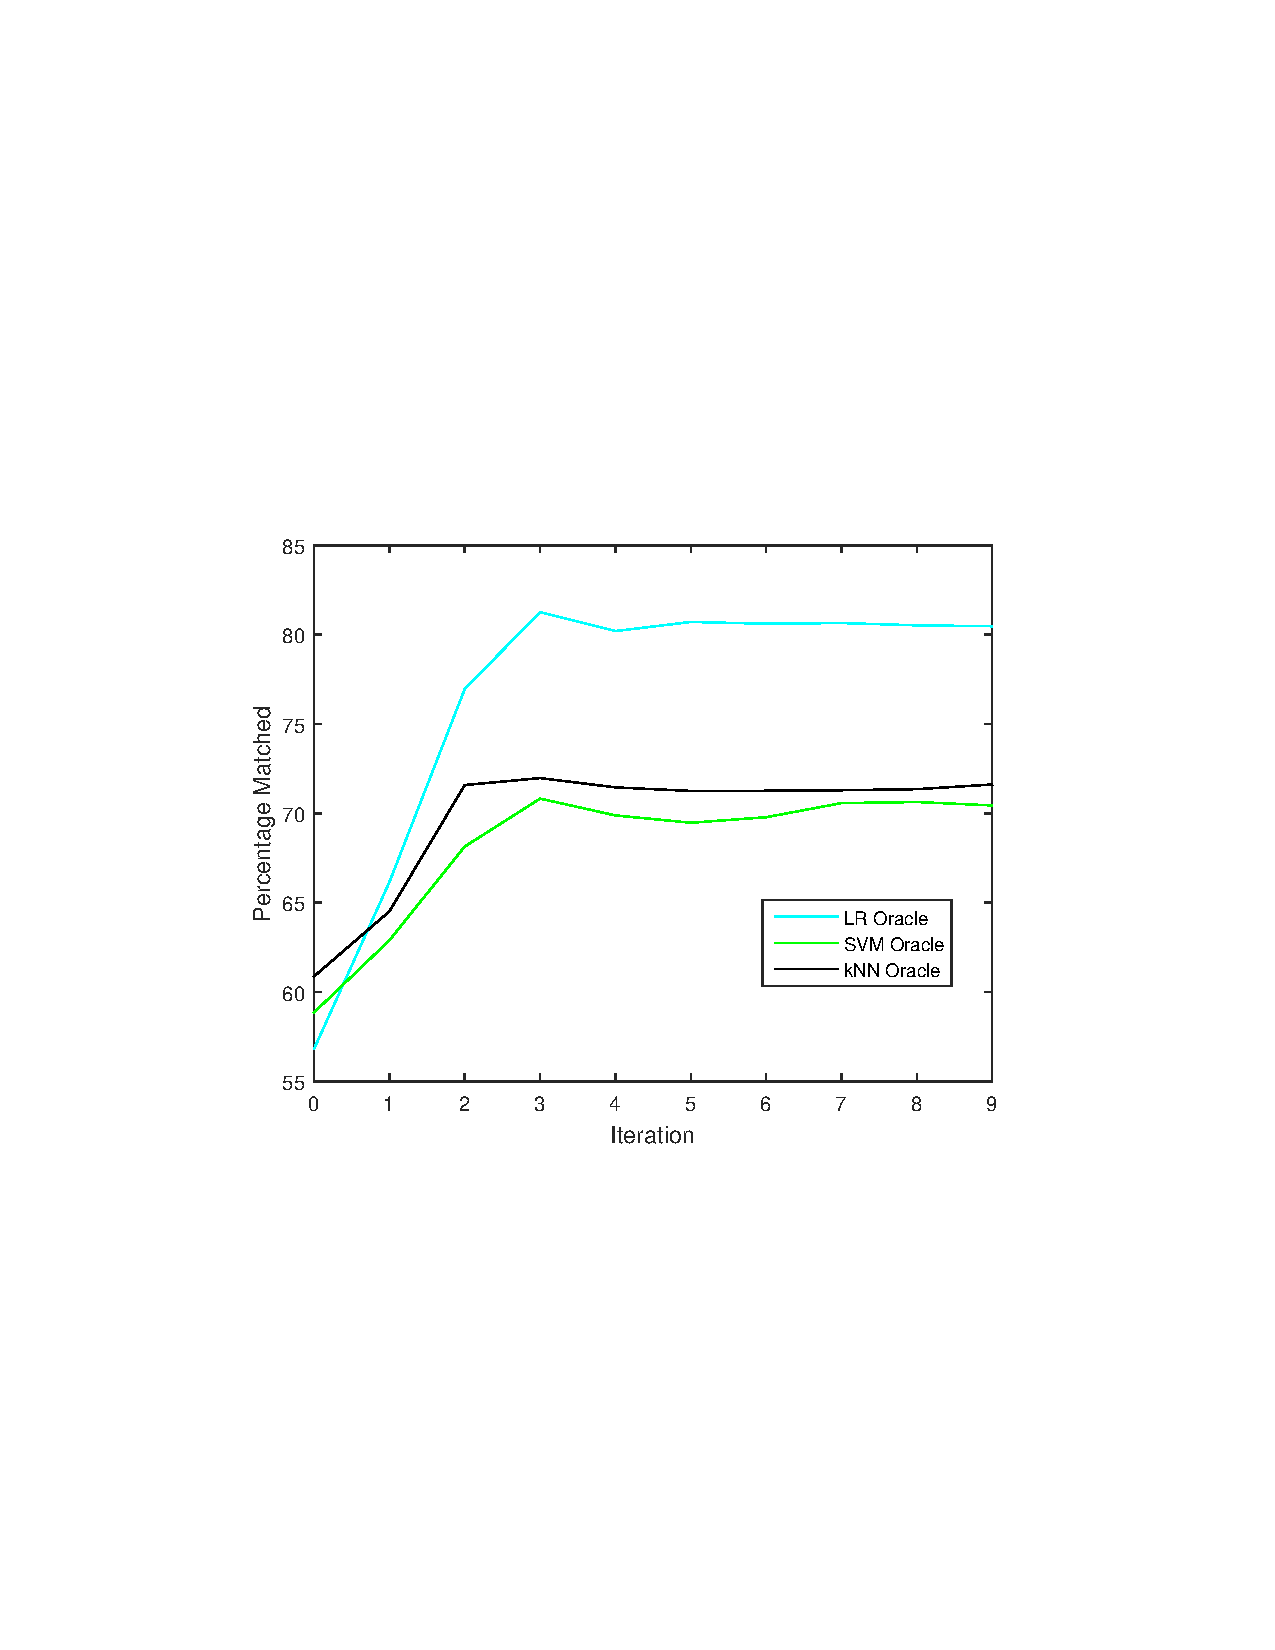
\includegraphics[width =\linewidth, trim = 110 240 120 255, clip]{figs/final_fig_1.pdf}
		\caption{Percentage of samples for which the substitute model and oracle classifications agree without feature reduction.}
		\label{fig:sub_approx}
	\end{minipage}
	\qquad
	\begin{minipage}{0.42\linewidth}
		\centering
		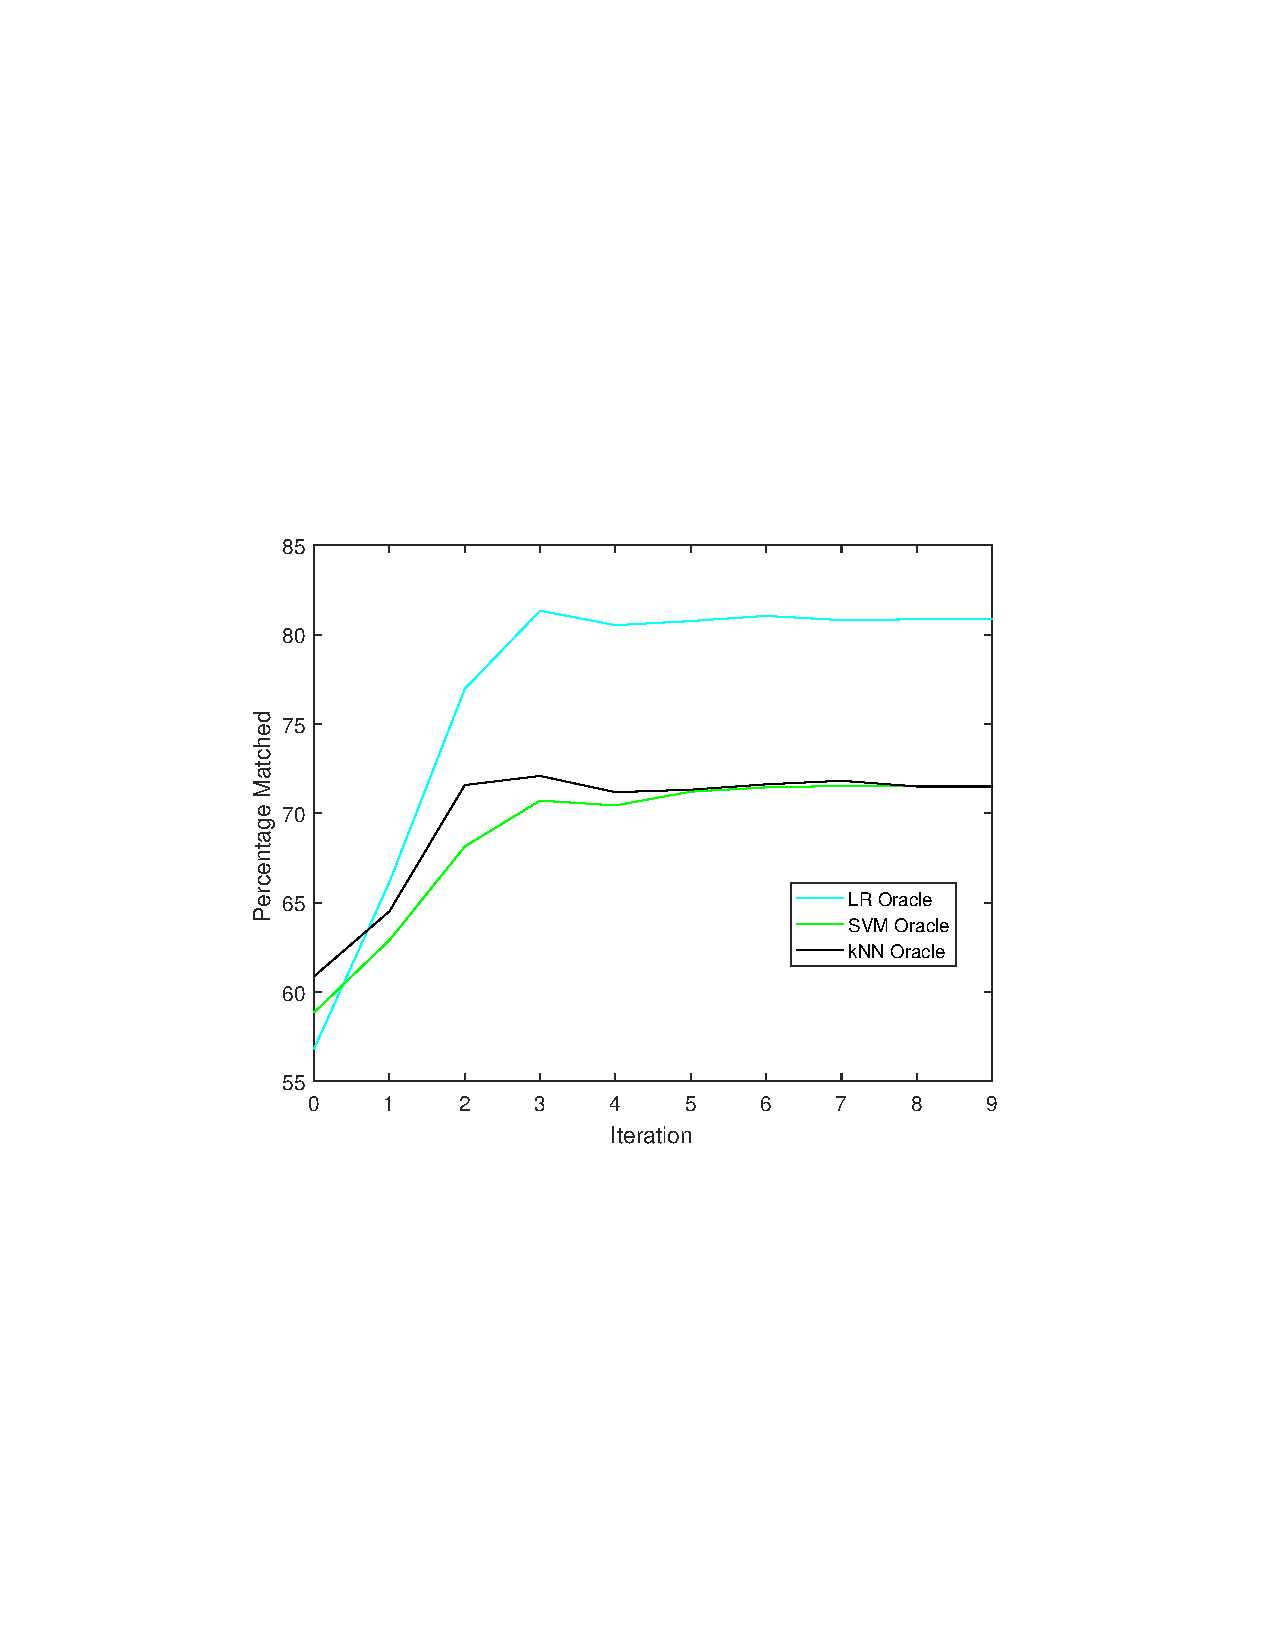
\includegraphics[width =\linewidth, trim = 110 240 120 255, clip]{figs/fig1_pca.pdf}
		\caption{Percentage of samples for which the substitute model and oracle classifications agree with PCA feature reduction.}
		\label{fig:sub_approx_pca}
	\end{minipage}
\end{figure*}

\begin{figure*}
	\centering
	\subfigure[Fast Gradient Descent Algorithm]{\label{fig:missclassify_fgs}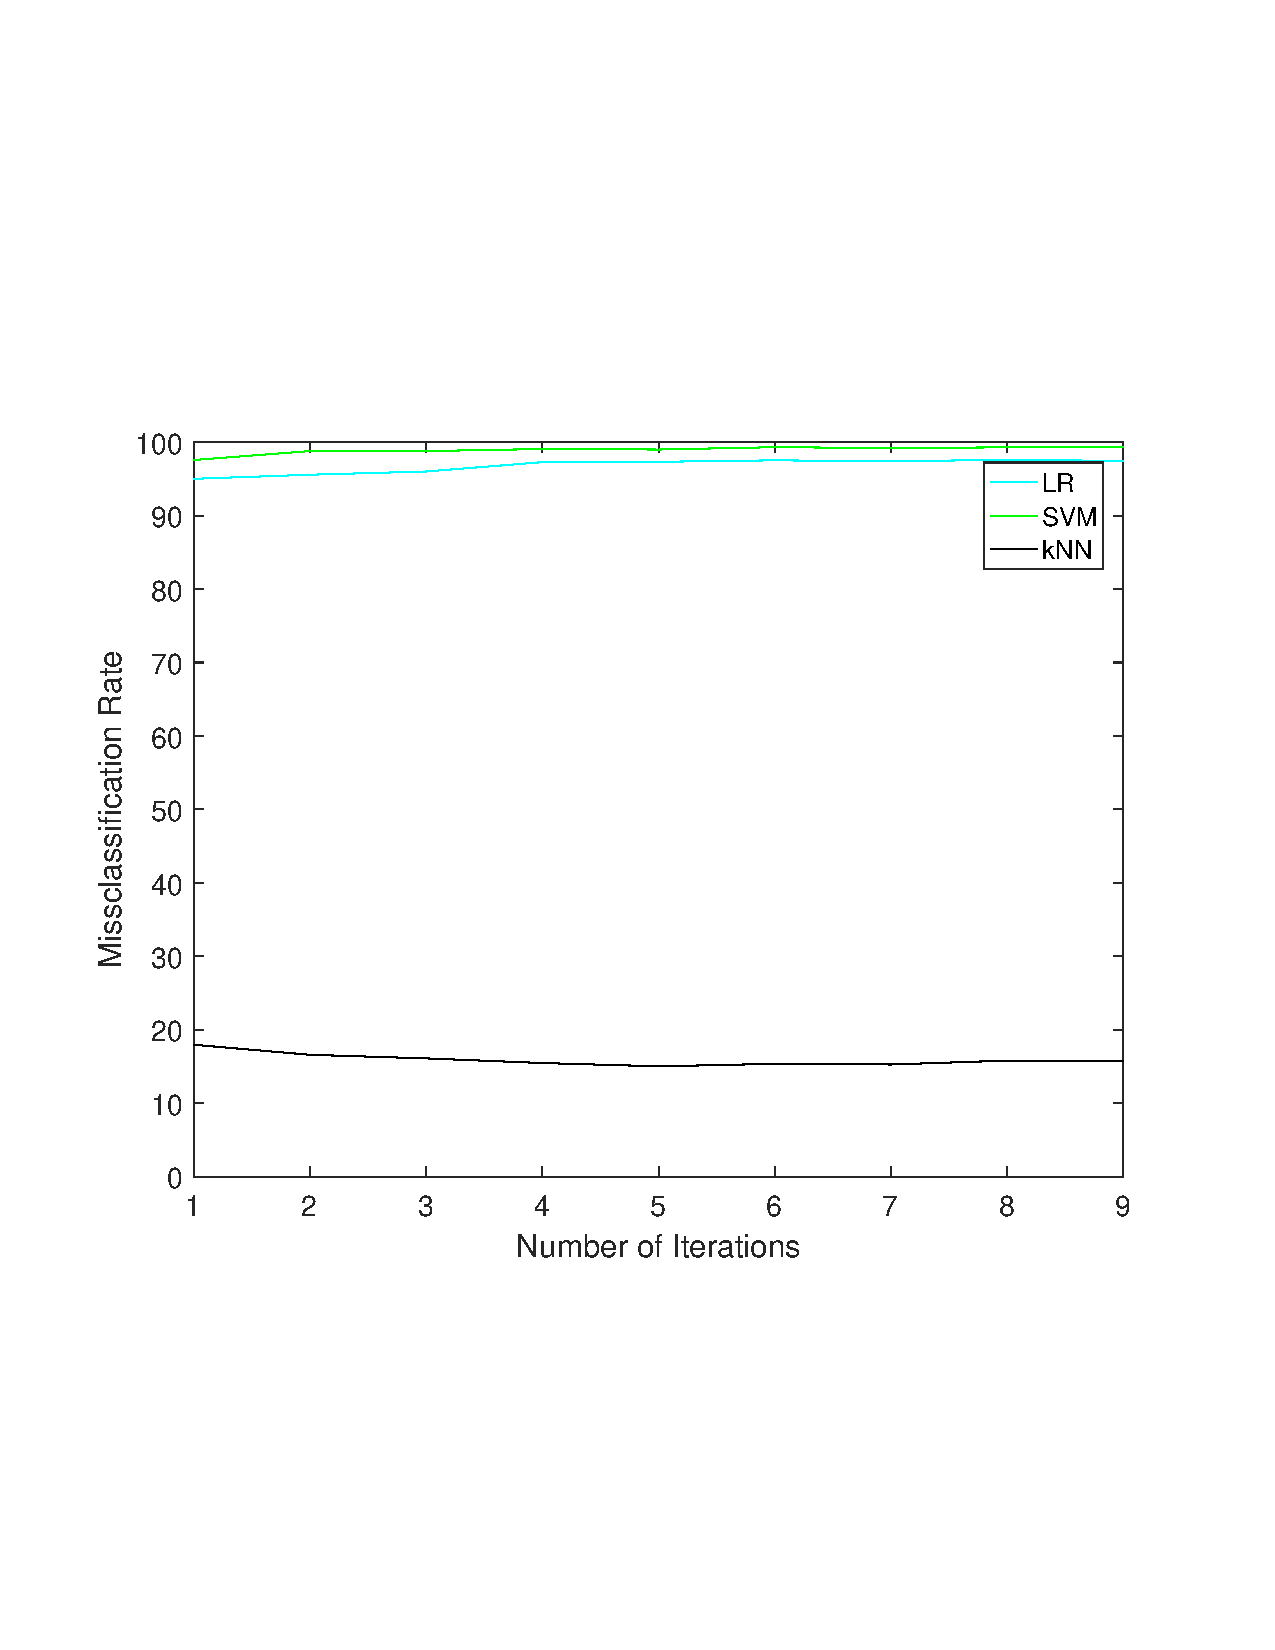
\includegraphics[width =0.4\linewidth, trim = 50 180 70 205, clip]{figs/misclass_goodfellow.pdf}}
	\qquad
	\subfigure[Papernot Algorithm]{\label{fig:missclassify_papernot}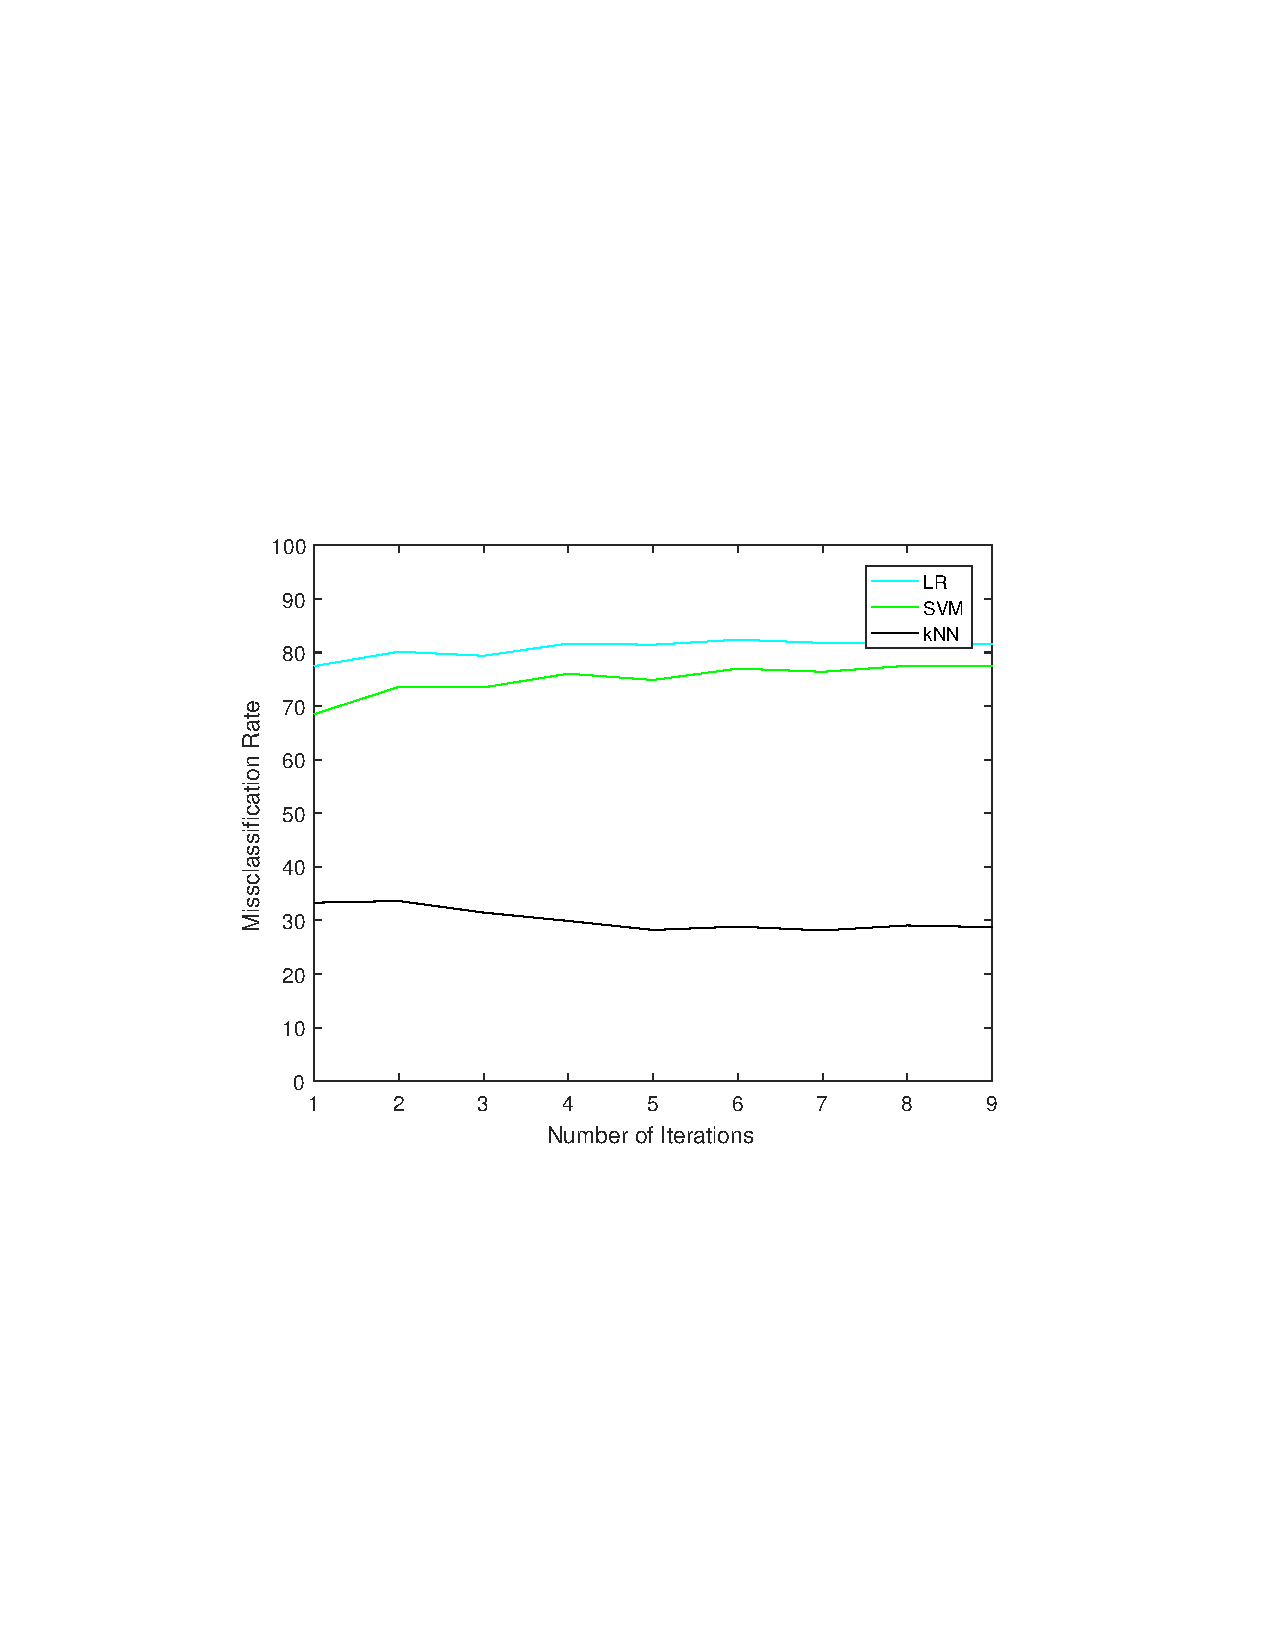
\includegraphics[width =0.415\linewidth, trim = 110 240 120 255, clip]{figs/missclass_papernot.pdf}}
	\caption{Misclassification rate vs. iteration of the Jacobian-based dataset augmentation without feature reduction}
\end{figure*}

\begin{figure*}
	\centering
	\subfigure[Fast Gradient Descent Algorithm]{\label{fig:missclassify_fgspca}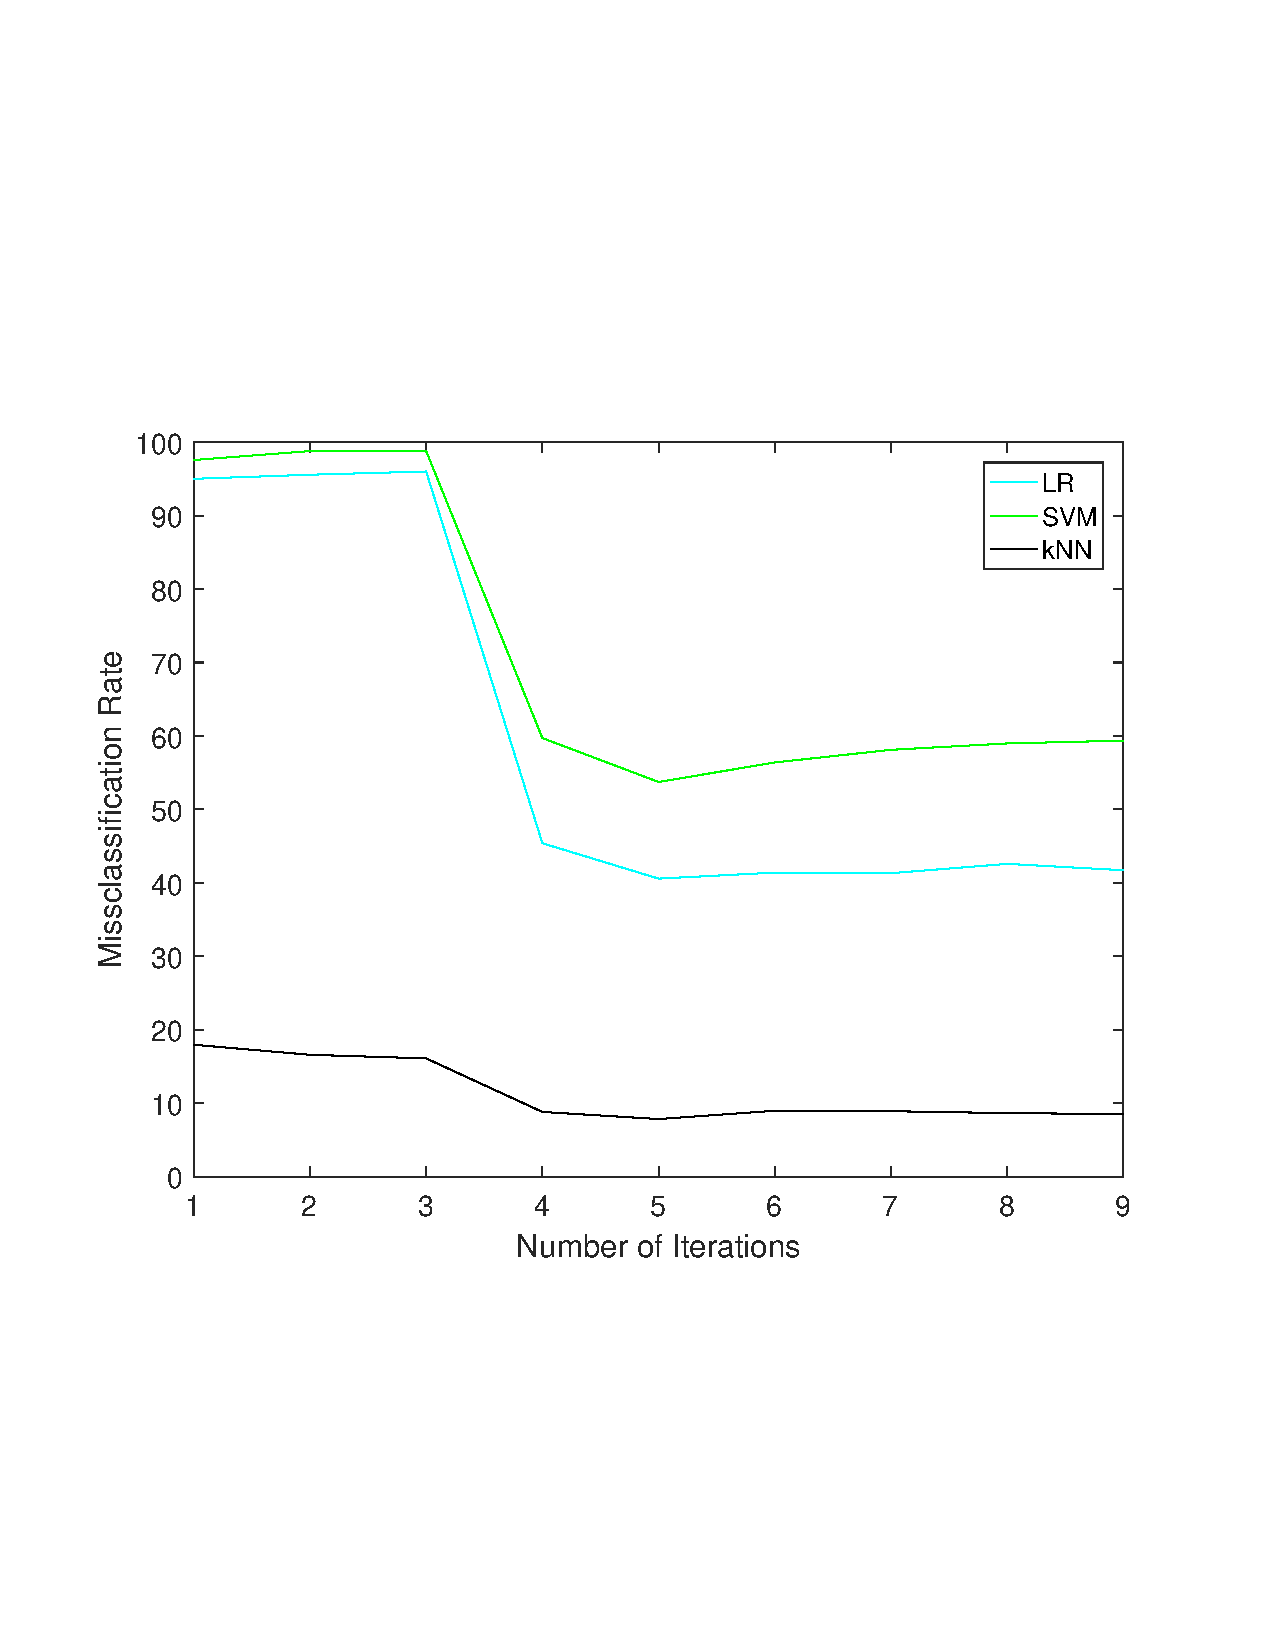
\includegraphics[width =0.4\linewidth, trim = 50 180 70 205, clip]{figs/misclass_goodfellow_pca.pdf}}
	\qquad
	\subfigure[Papernot Algorithm]{\label{fig:missclassify_papernotpca}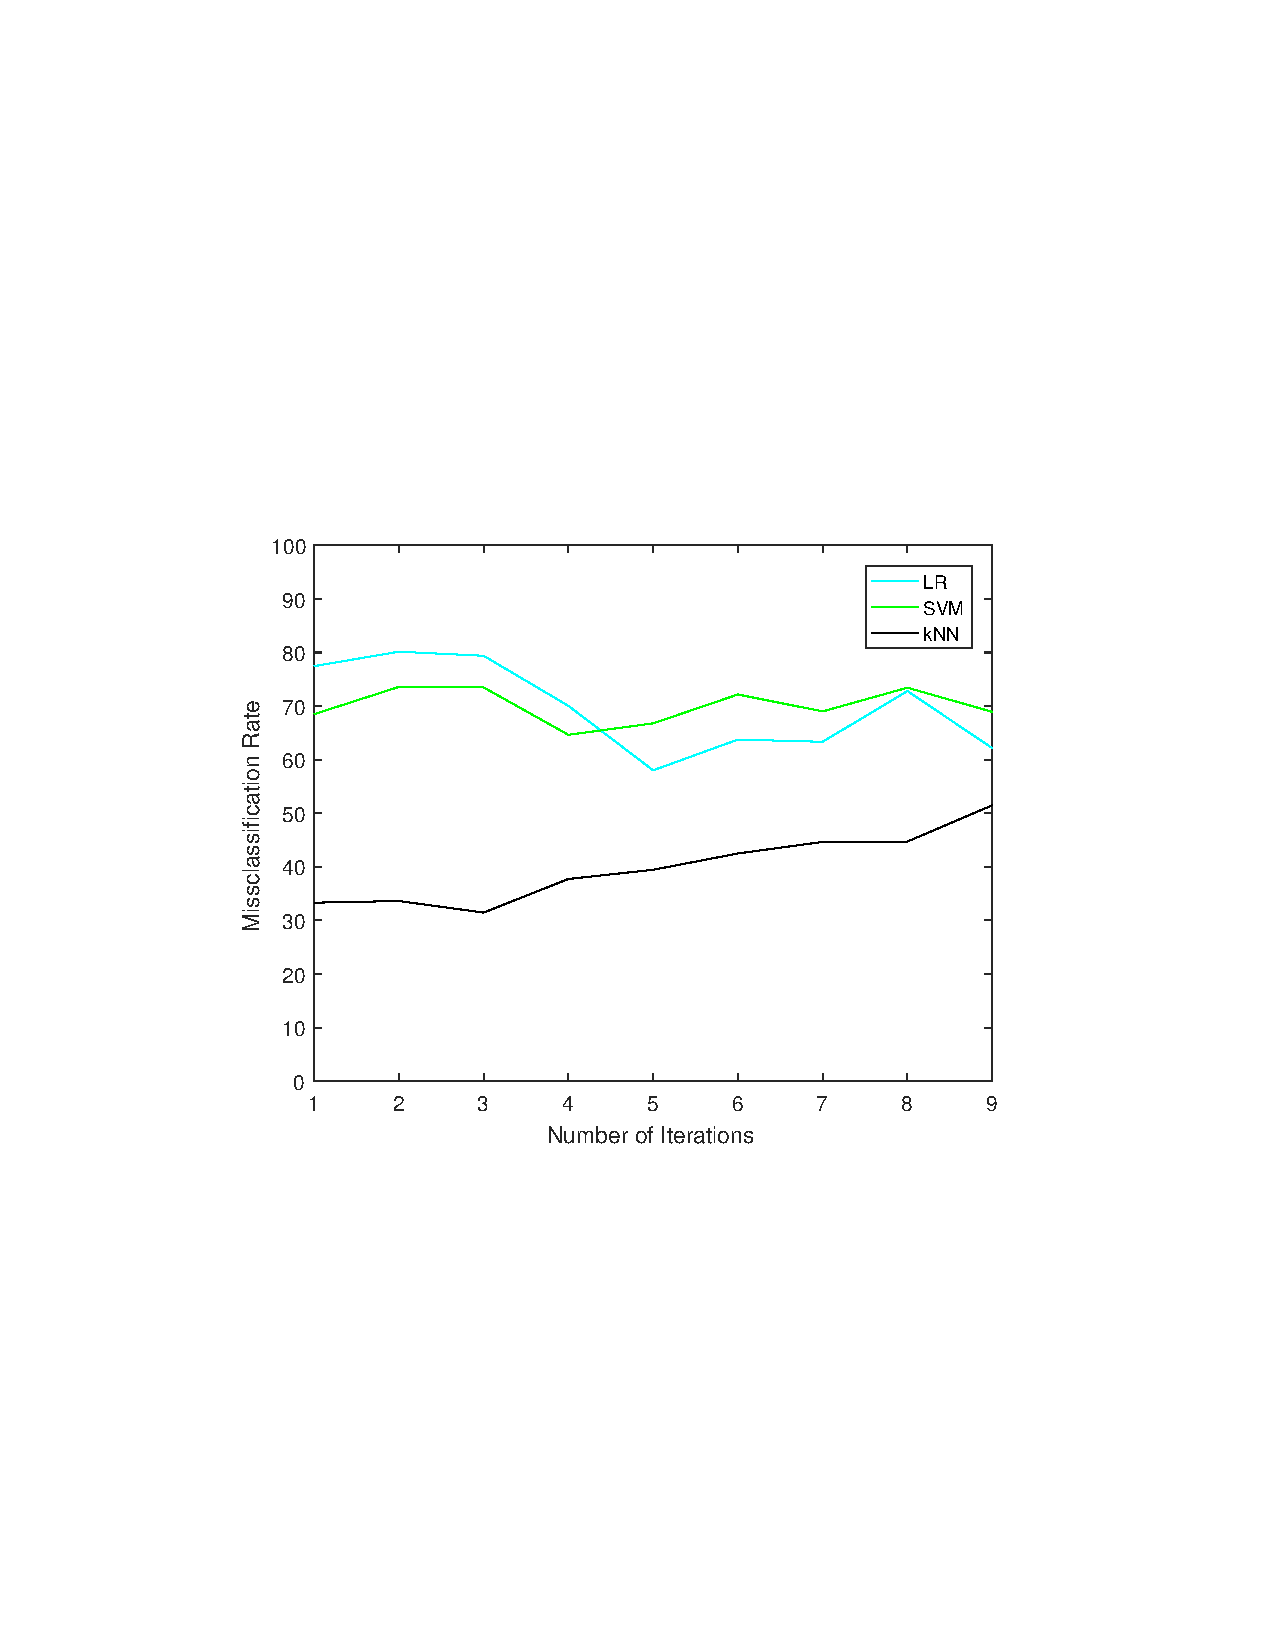
\includegraphics[width =0.415\linewidth, trim = 110 240 120 255, clip]{figs/missclass_papernot_pca.pdf}}
	\caption{Misclassification rate vs. iteration of the Jacobian-based dataset augmentation with PCA feature reduction}
\end{figure*}


\subsection{Performance of Crafted Adversarial Samples}
In our first experiment, we generated adversarial samples on the $10,000$ test samples based on the LR substitute model. The misclassification rates on the adversarial samples by the oracles are given in Figures \ref{fig:missclassify_fgs}  and \ref{fig:missclassify_papernot} for both the FGS and Papernot methods utilizing the full feature sets. To generate adversarial samples with FGS, we used $\epsilon = 0.3$ in Equation $\ref{eqn:fast_gradient_sign}$, which is the same value as that used in $\cite{papernot3}$. For the Papernot method, $10\%$ of the features (pixels) were perturbed for each image ($\gamma = 0.1$) with $\epsilon = 1$, similar to the parameters in \cite{papernot1}. \\
\indent In Figures \ref{fig:missclassify_fgs}  and \ref{fig:missclassify_papernot}, we were able to achieve fairly high misclassification rates for both the LR oracle and the SVM oracle, but performed poorly for the kNN oracle, which agrees with the results obtained by Papernot et al. $\cite{papernot3}$. Our misclassification rate was, in fact, slightly higher for all 3 models for the FGS method as reported in \cite{papernot3}, likely caused by the different gradient formulation utilized in our approach. The Papernot method performed notably worse than FGS due to intrinsically smaller perturbations. However, the Papernot parameters can be further tuned to achieve a desired balance between the misclassification rate and the amount of perturbation.\\
\indent In our second experiment, PCA feature-reduction was introduced at iteration 4 of the Jacobian-based dataset augmentation, when the training set size exceeded the number of features. Adversarial samples were generated by first carrying out FGS and Papernot algorithms on the reduced feature space and then restoring the samples as described in section \ref{sec:pca} before passing them into the oracle. The results are shown in Figures \ref{fig:missclassify_fgspca} and \ref{fig:confusion_matrix_papernotpca}. From Figure \ref{fig:missclassify_fgspca}, we can see that introducing PCA in the FGS algorithm dramatically decreased the misclassification rate. However, from Figure \ref{fig:missclassify_papernotpca}, the misclassification rate for the Papernot algorithm was only slightly impacted by the introduction of PCA, maintaining a reasonable misclassification rate of about $\sim 70\%$. For the kNN oracle, the rate even increased according to the figure. This suggests that PCA is a suitable feature reduction technique to use for the Papernot algorithm, specifically.\\
\indent To calculate the computational cost, we measured the time required to generate all $10,000$ of the adversarial samples in both experiments. The results are shown in Table \ref{tablewithstuff}. For the FGS algorithm, although there was a reduction in running time, the change was not significant, as FGS is already computationally efficient. For the Papernot algorithm, the reduction was substantial; the running time was cut by more than a factor of 2 for all three oracles. This suggests that PCA is successful at reducing the computational cost associated with the Papernot algorithm.\\
\indent The confusion matrices for the unaltered test images and the adversarial samples generated using the Papernot algorithm with PCA are shown in Figures \ref{fig:confusion_matrix_oracle} and \ref{fig:confusion_matrix_papernotpca}, respectively. The number in position $(i, j)$ of the grid corresponds to the percentage of class $i$ images being classified as class $j$. The Papernot algorithm with PCA was generally successful at misdirecting the oracle, except for the numbers "1" and "6" (darker squares in Figure \ref{fig:confusion_matrix_papernotpca}), which were robust to the attack. The precision, recall, and accuracy for all test samples and adversarial samples are displayed in Table \ref{tablewithstuff}, presenting the same trends as in the confusion matrices.\\
\indent A single unaltered image and its associated sample adversarial images are shown in Figure \ref{fig:picof9s}. Both the SVM oracle and the LR oracle misclassified the perturbed images. We can see that these images are still easily recognizable as a "9", so the adversarial attacks were successful. However, the deviations added to the image are also clearly visible to the human eye, which is undesirable. These deviations could be reduced with further parameter tuning and higher resolution images. Note that, as expected, the deviations added to the image were less noticeable in the Papernot algorithm as compared to that of the FGS method. 

%This explains why Papernot algorithm was found to have a lower misclassification rate than FGS algorithm.

%We implemented the above algorithm utilizing a reduced image feature set. Specifically, we reduced each of the $28 \times 28$ pixel images in the LR substitute model training set by a \textbf{factor of 8}.

\begin{figure}
    \centering
    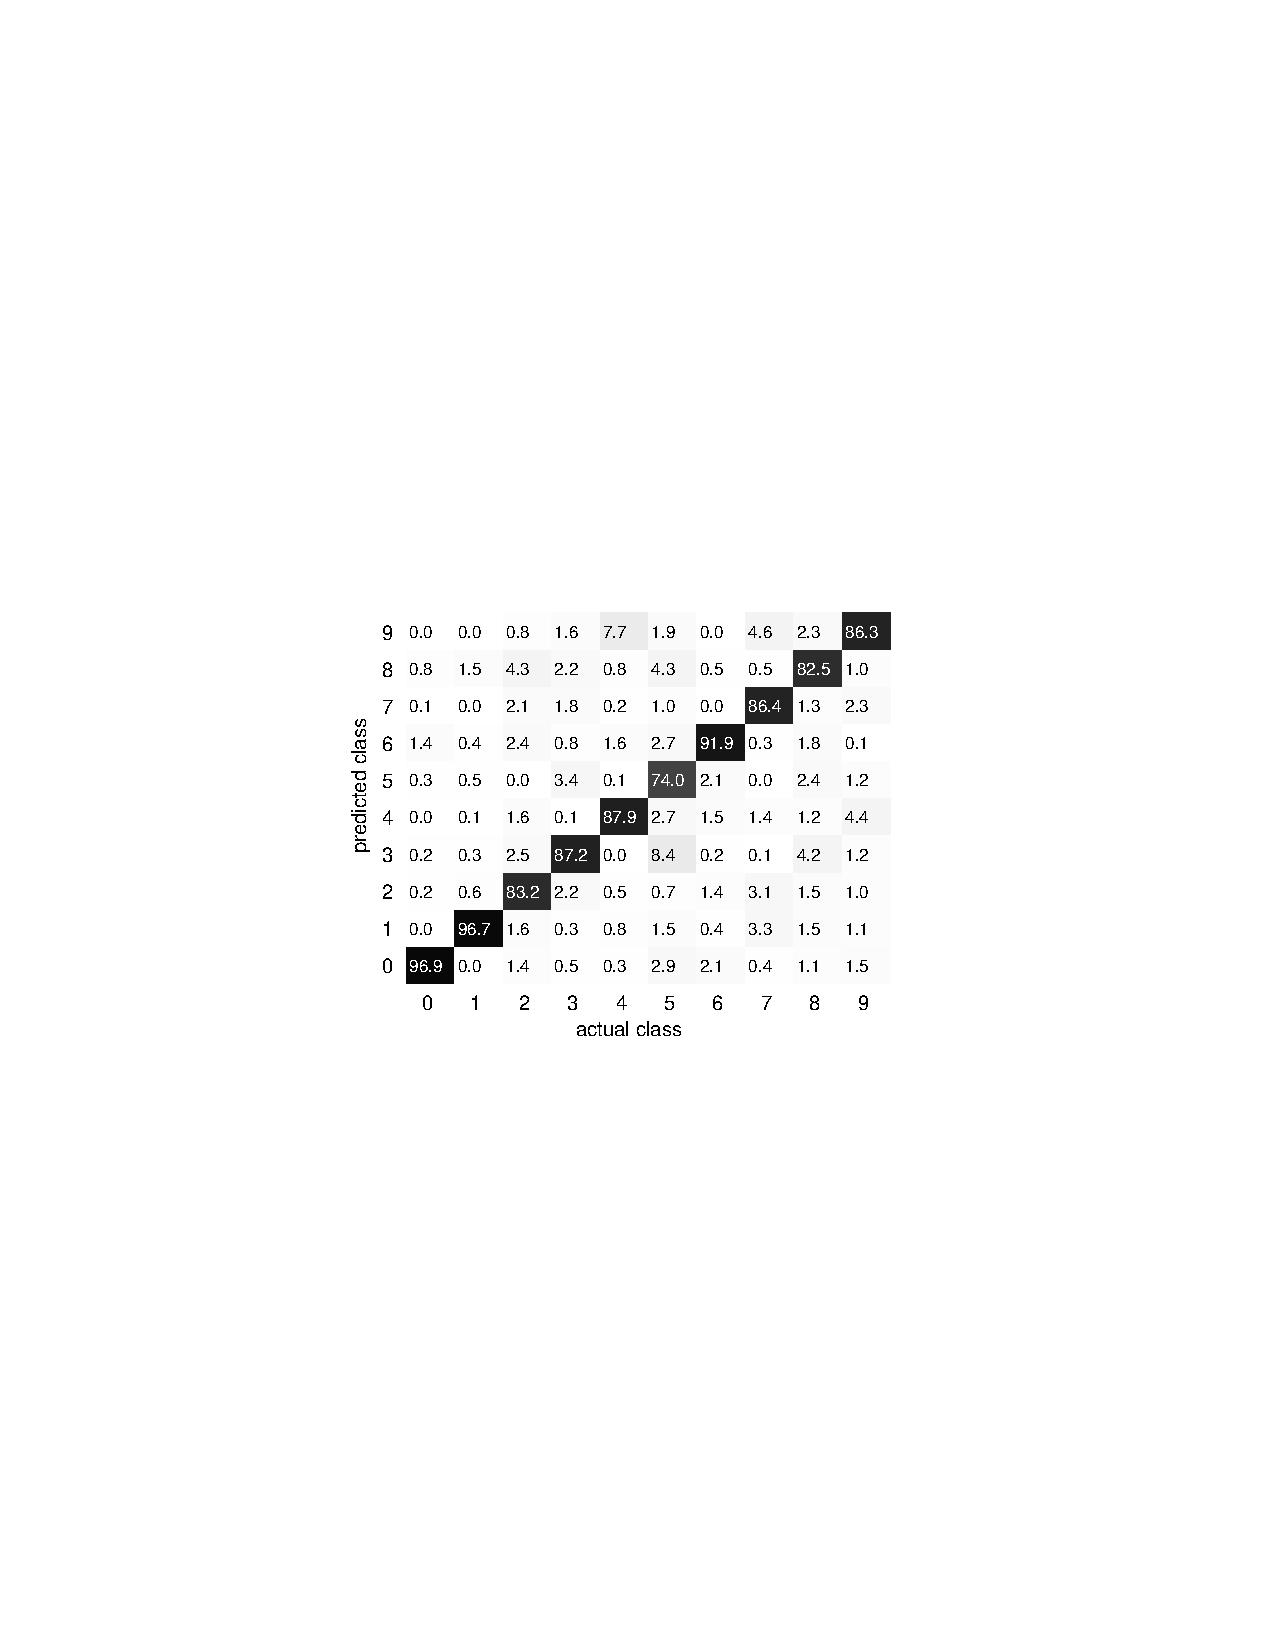
\includegraphics[width =\linewidth, trim = 120 295 150 280, clip]{figs/confusion_matrix_oracle.pdf}
    \caption{Confusion matrix against the LR oracle for the original 10,000 test samples.}
    \label{fig:confusion_matrix_oracle}
\end{figure}

\begin{figure}
    \centering
    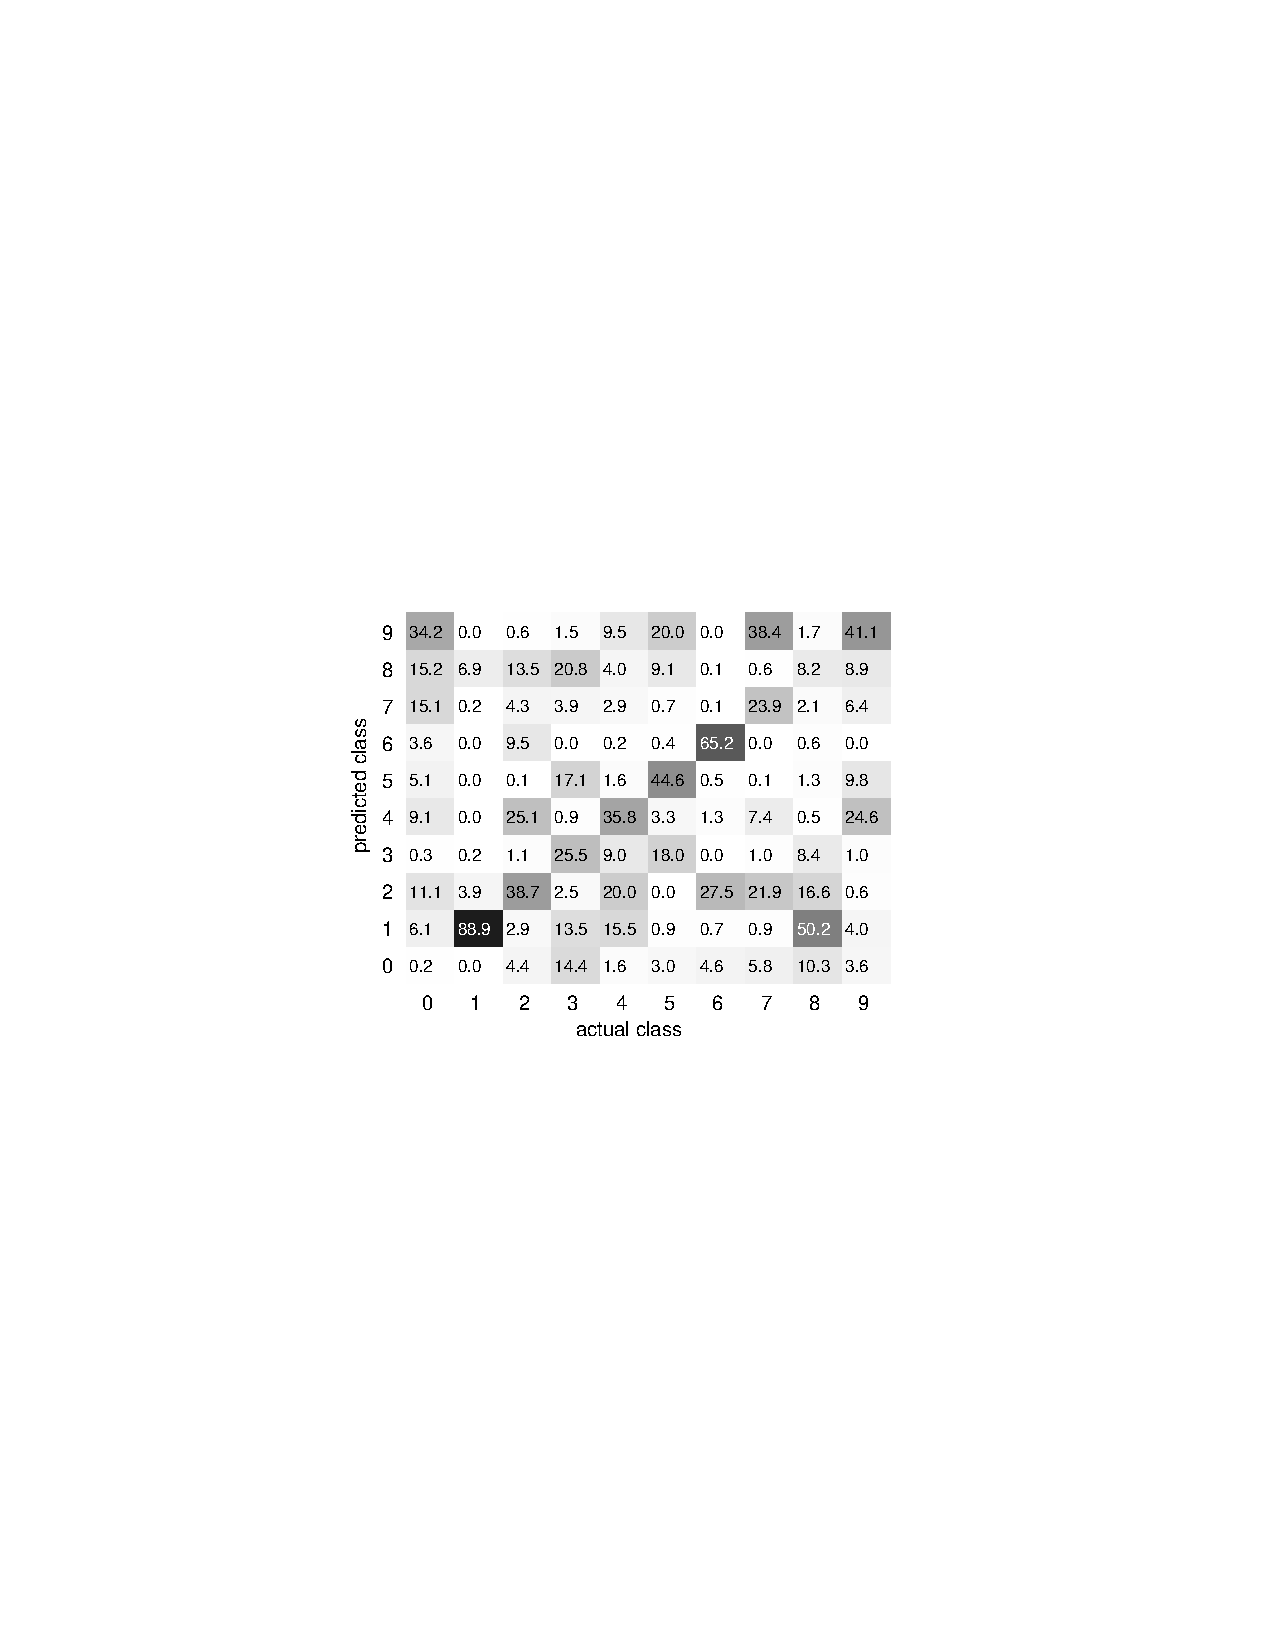
\includegraphics[width =\linewidth, trim = 120 295 150 280, clip]{figs/confusion_matrix_papernotpca.pdf}
    \caption{Confusion matrix against the LR oracle for the 10,000 adversarial samples generated using the Papernot method with PCA.}
    \label{fig:confusion_matrix_papernotpca}
\end{figure}

\begin{table}[t]
	\caption{Runtime for generating 10,000 adversarial samples in seconds for the three oracle models using FGS.}
	\label{runtime_FGS}
	\vskip 0.15in
	\begin{center}
		\begin{small}
			\begin{sc}
				\begin{tabular}{lccr}
					\hline
					\abovespace\belowspace
					&LR & SVM & kNN\\
					\hline
					\abovespace
					FGS & 1.3912 & 1.5692 & 1.7441 \\
					FGS + PCA & 1.3509 & 1.2557 & 1.3681\\				
					\hline
				\end{tabular}
			\end{sc}
		\end{small}
	\end{center}
	\vskip -0.1in
\end{table}

\begin{table}[t]
	\caption{Runtime for generating 10,000 adversarial samples in seconds for the three oracle models using Papernot method.}
	\label{runtime_Papernot}
	\vskip 0.15in
	\begin{center}
		\begin{small}
			\begin{sc}
				\begin{tabular}{lccr}
					\hline
					\abovespace\belowspace
					&LR & SVM & kNN\\
					\hline
					\abovespace
					Papernot & 7.9147 & 7.9776 & 8.57\\
					Papernot + PCA & 3.1826 & 3.0719 & 3.3997\\				
					\hline
				\end{tabular}
			\end{sc}
		\end{small}
	\end{center}
	\vskip -0.1in
\end{table}

\begin{table}[t]
	\caption{Average precision, recall, and accuracy for the original test images and adversarial images constructed using Papernot algorithm with PCA.}
	\label{tablewithstuff}
	\vskip 0.15in
	\begin{center}
		\begin{small}
			\begin{sc}
				\begin{tabular}{lccc}
					\hline
					\abovespace\belowspace
					&Precision & Recall & Accuracy\\
					\hline
					\abovespace
					Original & 87.4645 &  87.3036  & 87.5300 \\
					Adversarial & 37.3687 &  37.2288 &  37.8400\\				
					\hline
				\end{tabular}
			\end{sc}
		\end{small}
	\end{center}
	\vskip -0.1in
\end{table}

\begin{figure}
\centering
\begin{minipage}{.09\textwidth}
	\centering
    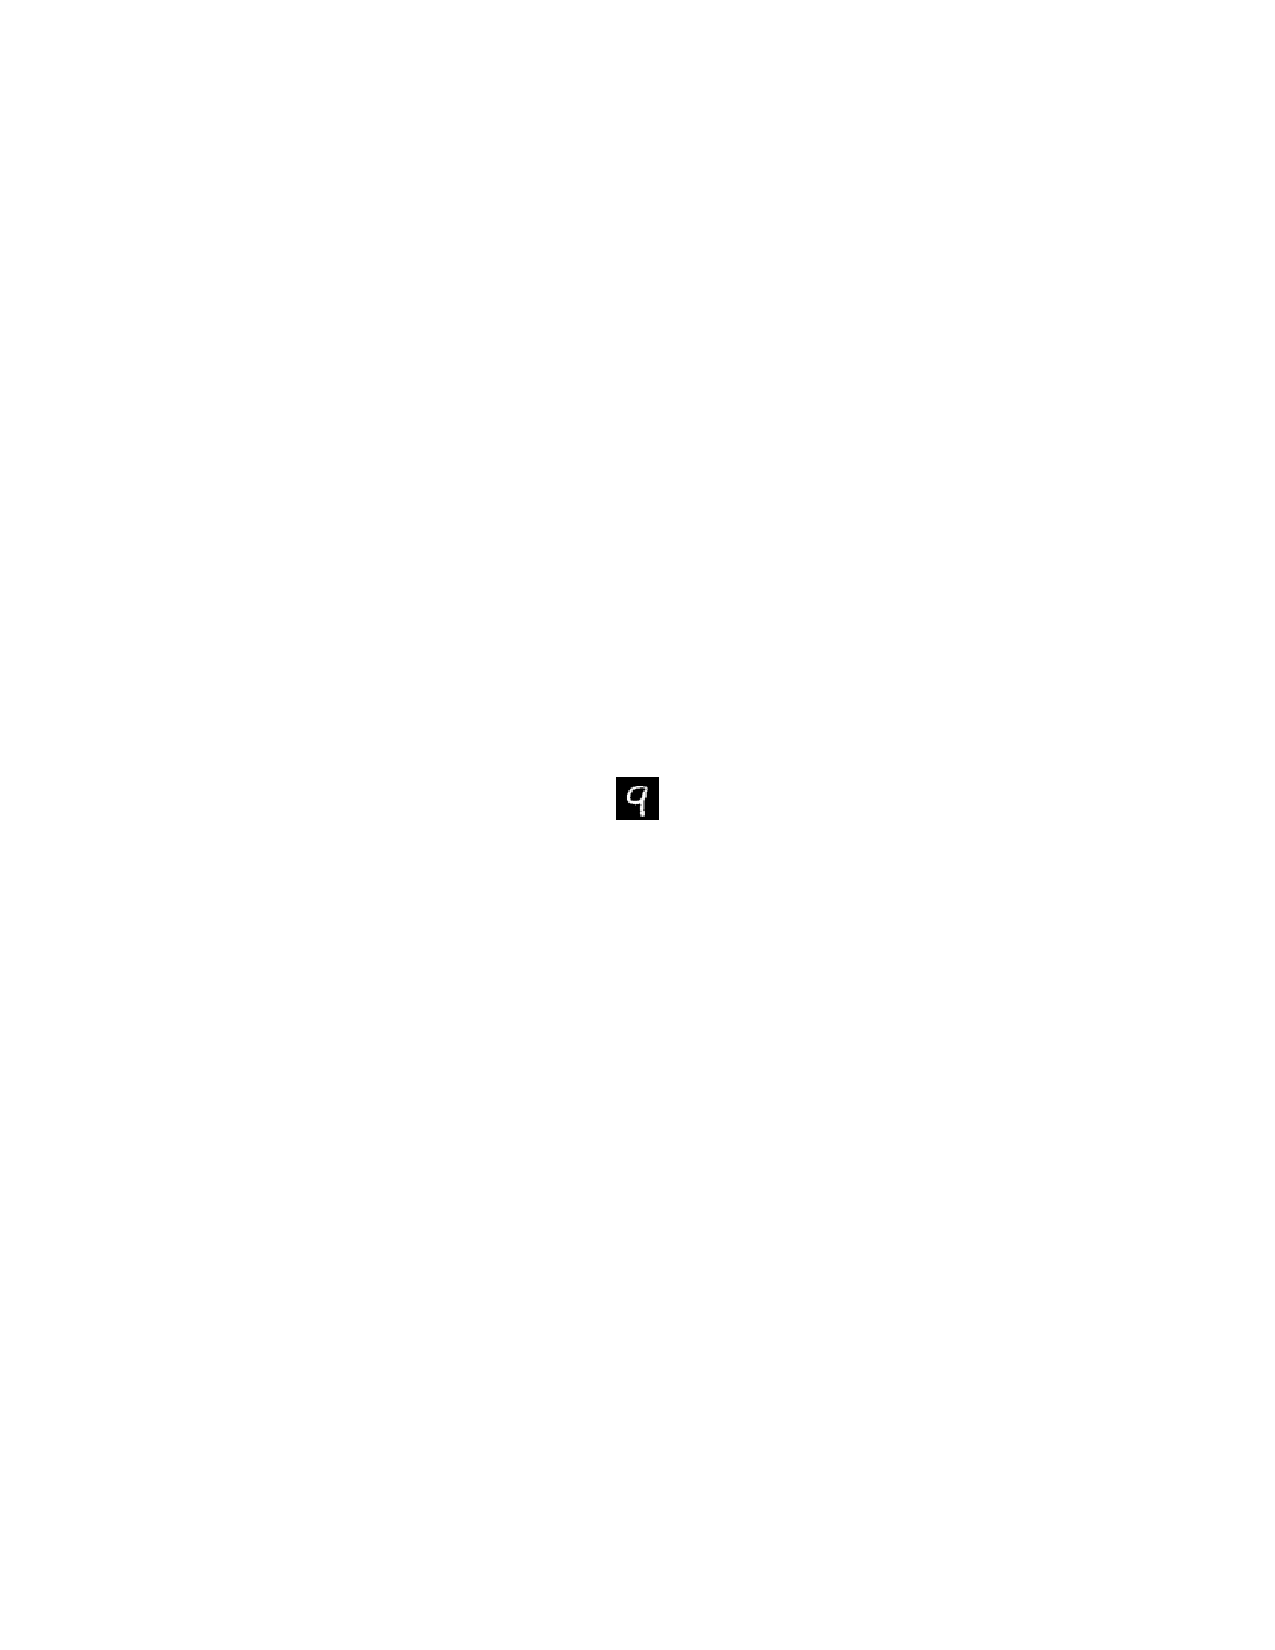
\includegraphics[width =0.9\linewidth, trim = 300 400 300 375, clip]{figs/orig9.pdf}
\end{minipage}%
\begin{minipage}{.09\textwidth}
	\centering
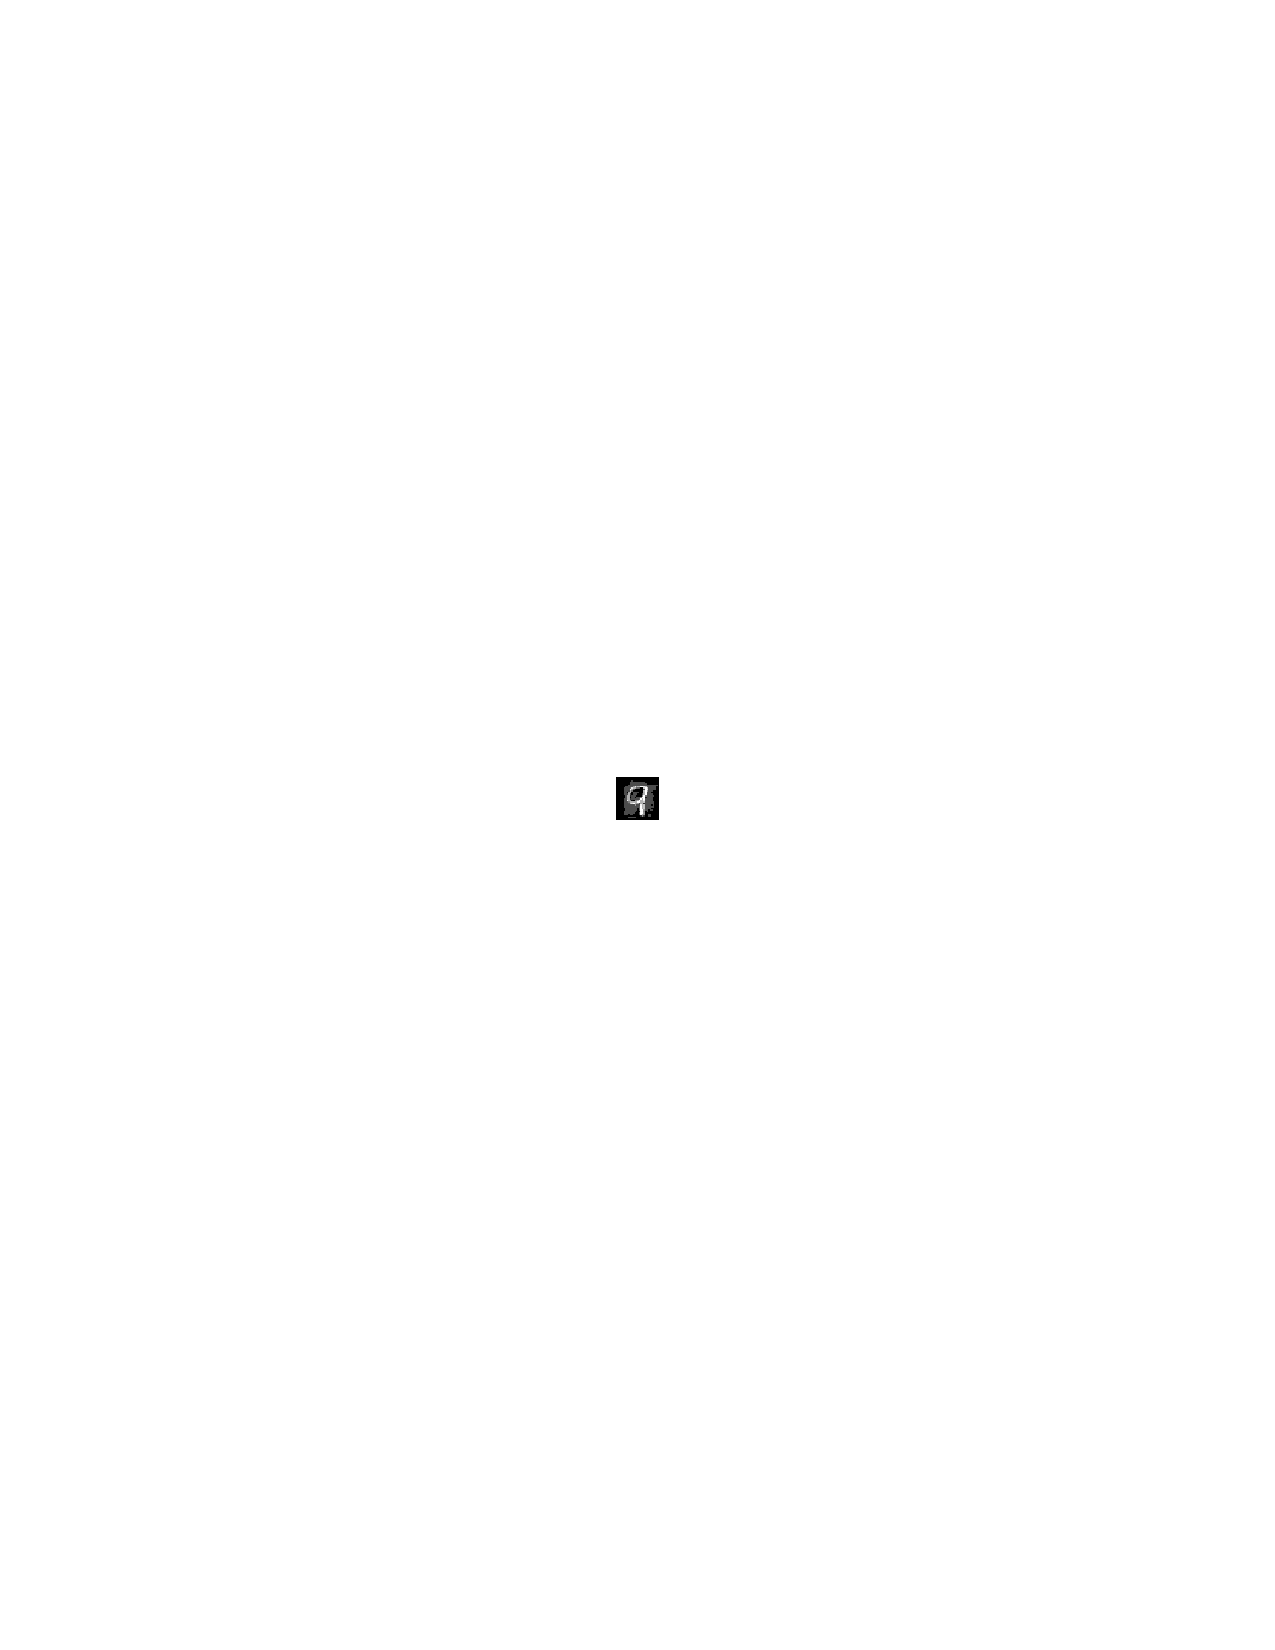
\includegraphics[width =0.9\linewidth, trim = 300 400 300 375, clip]{figs/goodfellow9.pdf}
\end{minipage}
\begin{minipage}{.09\textwidth}
	\centering
    
\includegraphics[width =0.9\linewidth, trim = 300 400 300 375, clip]{figs/goodfellow9pca.pdf}
\end{minipage}
\begin{minipage}{.09\textwidth}
	\centering
    
\includegraphics[width =0.9\linewidth, trim = 300 400 300 375, clip]{figs/papernot9.pdf}
\end{minipage}
\begin{minipage}{.09\textwidth}
	\centering
    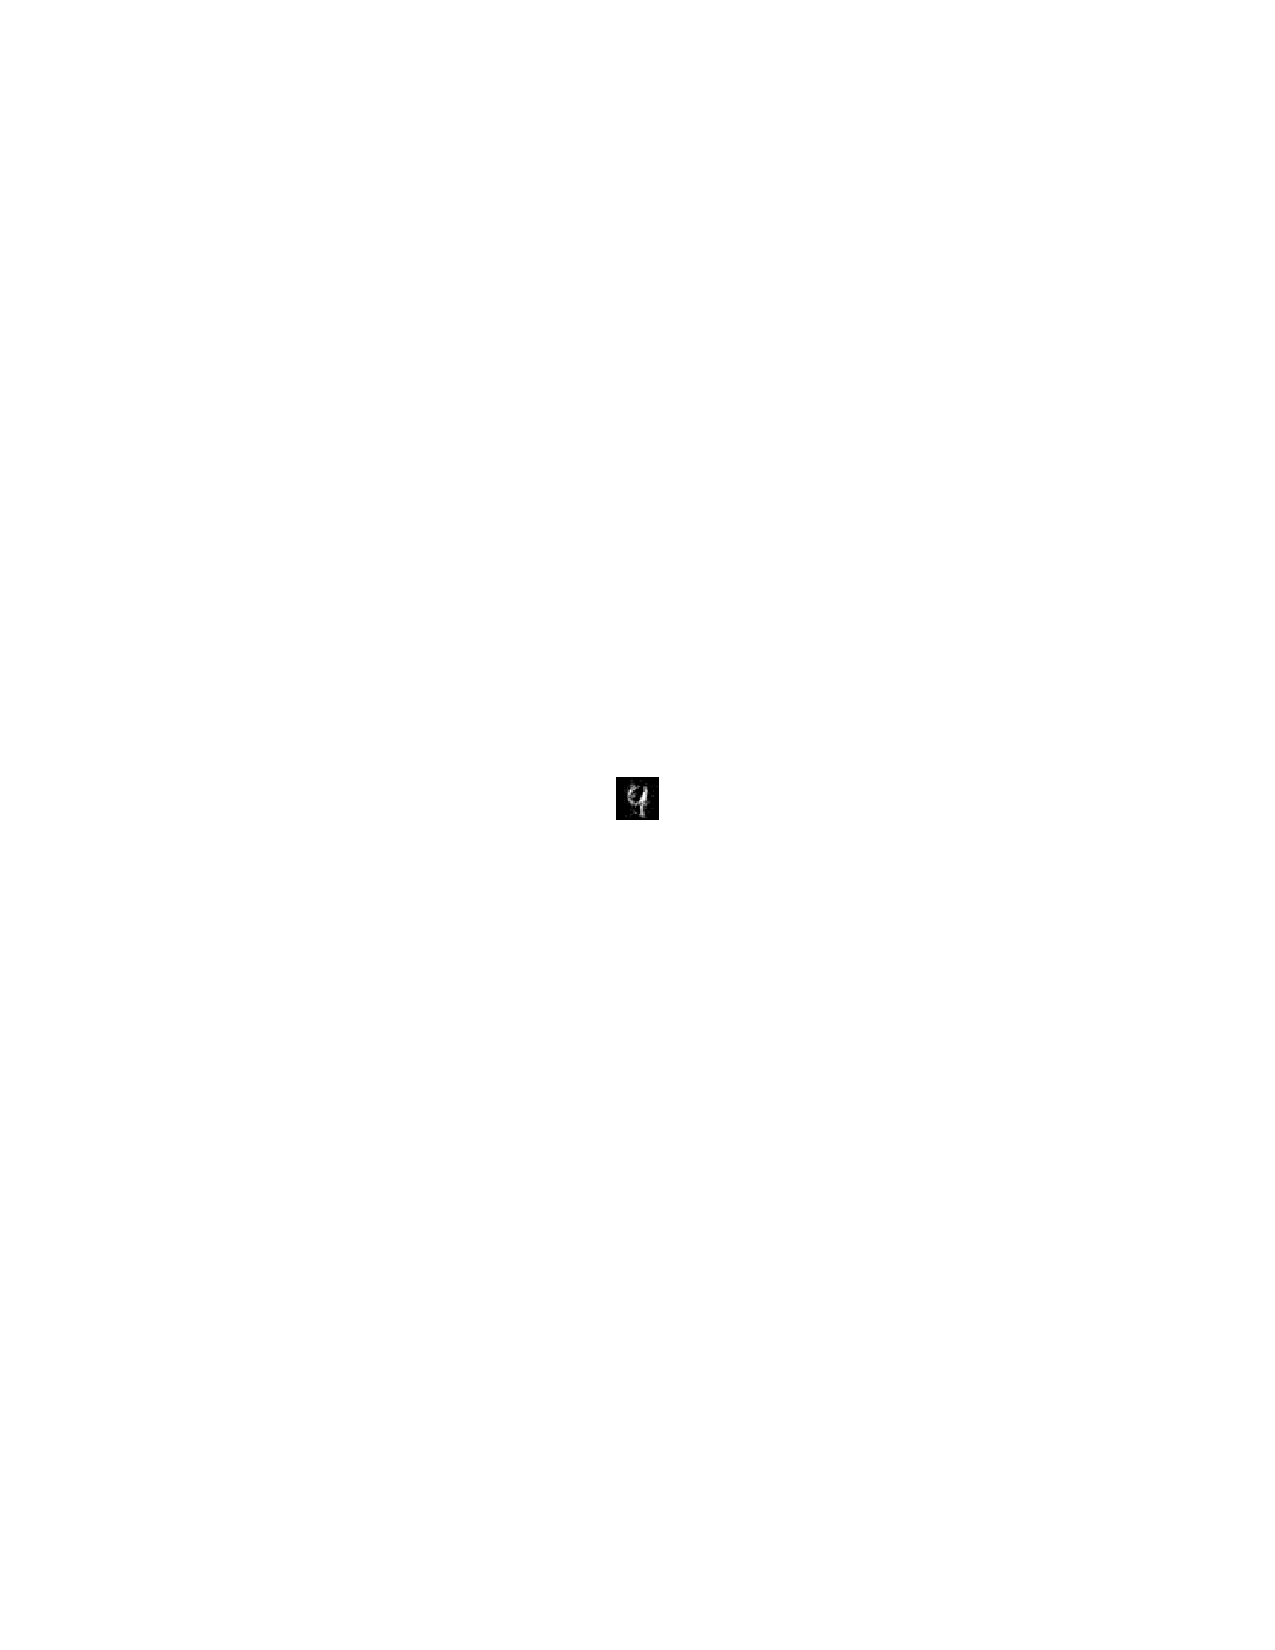
\includegraphics[width =0.9\linewidth, trim = 300 400 300 375, clip]{figs/papernot9pca.pdf}
\end{minipage}
\caption{From left to right, the figures are: original image, adversarial image with FGS method, adversarial image with FGS method and PCA feature reduction, adversarial image with Papernot method, adversarial image with Papernot method and PCA.}\label{fig:picof9s}
\end{figure}
	\section{CONCLUSIONS and FUTURE WORK}

% We have shown that the computational efficiency of adversarial attacks on machine learning classifiers is improved with the implementation of PCA, which reduces the feature dimensionality by a factor of $8$.
%The method followed in this paper is two-fold. 
We attacked image classifiers using a two fold strategy: we first imitated the target classifier with a substitute LR model and then generated adversarial samples based on the substitute model \cite{papernot3}. To reduce the computational cost of crafting adversarial samples, we reduced the feature space dimensionality by utilizing PCA. Although PCA reduced the performance of the adversarial samples in FGS, it only had a small impact on the success of the Papernot algorithm, maintaining a reasonable misclassification rate of about $\sim 70\%$. Furthermore, although the runtime reduction due to PCA was negligible for FGS, it was significant for the Papernot algorithm, reducing the computation time by half. We have shown that we can increase the efficiency of adversarial sample construction while maintaining misclassification effectiveness utilizing the Papernot adversarial sample crafting method in combination with PCA feature reduction. 

%We found that PCA seemed to improve the quality of adversarial images for the FGS method, but compromised the quality of the adversarial images for the Papernot method. 

%The performance of the adversarial samples, although diminished, is still acceptably effective after introducing PCA to reduce the feature space. 

%Since the dimensionality reduction proved to be generally successful on the MNIST dataset, improving the efficiency of Papernot's algorithm in \cite{papernot3}, then 
For future work, the same approach could be applied to more complex images such as the GTSRB dataset of coloured traffic signs. The GTSRB images have a higher resolution, allowing for the perturbations added to the samples to be more subtle. Furthermore, the algorithm presented in this paper should be extended to targeted misclassification. These additions would portray the inherent vulnerability of machine learning algorithms to adversarial attacks in such high-risk applications as autonomous car navigation (e.g. having the oracle read a stop sign as a yield sign \cite{papernot1}). 
	\bibliography{references}
	\bibliographystyle{icml2017}
\end{document}